\section{Ensemble Learning}
\begin{definition}[Ensemble methods]
\textbf{Ensemble methods} (also known as classifier combination methods) are used to improve classification accuracy by aggregating the predictions of multiple classifiers. An ensemble method constructs a set of \textbf{base classifiers} trained on the training set (sampled differently depending on the technique), and then predicts the output on instances via majority vote.
\end{definition}
The key idea that justifies the use of ensemble methods is the so-called \hyperlink{https://en.wikipedia.org/wiki/The_Wisdom_of_Crowds}{\textbf{wisdom of the crowds}}: the collective knowledge of a diverse and independent group of people usually exceeds that of a single individual. According to Surowiecki, five elements are required to form a wise crowd: \textit{diversity of opinion}, \textit{independence} (a person's prediction is not influenced by the others in the crowd), \textit{decentralization} (people have specialization and local knowledge), \textit{aggregation} (a mechanism combines all predictions into a single one), and \textit{trust}. The same elements carry over to machine learning, where each \textit{individual} in the crowd is a \textit{model}.

Ensemble classifiers can be constructed in many ways:
\begin{itemize}
    \item By manipulating the training set (\textit{bagging}, \textit{boosting});
    \item By manipulating the input features, i.e., providing to the classifier different sets of columns (\textit{random forests});
    \item By manipulating the class labels (\textit{error-correcting output coding}).
\end{itemize}

\subsection{Bootstrap Aggregating (Bagging)}
\textbf{Bagging} is a technique that samples with replacement from a data set according to a probability distribution. Given a dataset $X = \{x_1, \dots, x_n \}$, bagging samples $m$ datasets of size $n$, say $\{X_1^*,..,X_m^*\}$, such that each record $x_i$ in each bootstrap extraction has the same probability of being extracted ($\frac{1}{n}$).

In the following pseudocode, $\delta()$ is a function that returns 1 if its argument is true, 0 otherwise.
\begin{algorithm}[H]
\caption{Bagging algorithm.}
\begin{algorithmic}[1]
    \State Let $k$ be the number of bootstrap samples.

    \For{$i=1$ to $k$}
        \State $D_i$ = Sample of size $N.\;\;$ $\#$ each sample has $P= 1/n$ to be selected
        \State Train a base classifier $C_i$ on $D_i$.
    \EndFor
    \State $C^*(x) = \arg\max_y \sum_i \delta(C_i(x) = y)\;\;$ \Comment{math way to say majority voting}
\end{algorithmic}
\end{algorithm} 
Bagging improves the generalization error by reducing the variance of the base classifiers. If a base classifier is unstable, bagging helps to reduce the errors associated with fluctuations in the training data, and if it is stable, the error of the ensemble will be mainly caused by bias of the base classifier.

\subsection{Boosting}
\textbf{Boosting} is an iterative procedure that changes the distribution of training examples for the base classifiers, raising the weight of instances that are harder to learn.

Initially, every instance in the original dataset is assigned a weight equal to $\frac{1}{n}$; a sample is drawn (as in bagging, with replacement), and a classifier is built on it. Every \textit{incorrectly classified} record has its weight increased, so it becomes more likely to be chosen in subsequent rounds.

For the next step, another sample is obtained considering the new weights, and used to train a second model. After classifying those instances, their weights are updated, and this goes on until the desired number of boosting rounds is reached.

\subsubsection{AdaBoost}
\textbf{AdaBoost} assigns to each base classifier $C_i$ an \textbf{importance} based on the classifier's error rate $\varepsilon_i$:
\begin{equation}
    \varepsilon_i = \sum_{j=1}^l w_j \delta(C_i(x_j) \neq y_j) \qquad \text{classifier's error rate} \label{AdaErrorRate}
\end{equation}
where $\delta()$ is the same function seen in the bagging pseudocode, but here it returns 1 when the condition holds (the classifier's prediction on $j$ differs from the expected label), which contributes to increasing the weight. The importance is then computed as:
\begin{equation}
    \alpha_i = \dfrac{1}{2} \ln \left(\dfrac{1-\varepsilon_i}{\varepsilon_i}\right) \quad\text{importance}\label{AdaImportance}
\end{equation}

\begin{wrapfigure}{r}{0.3\linewidth}
    \centering
    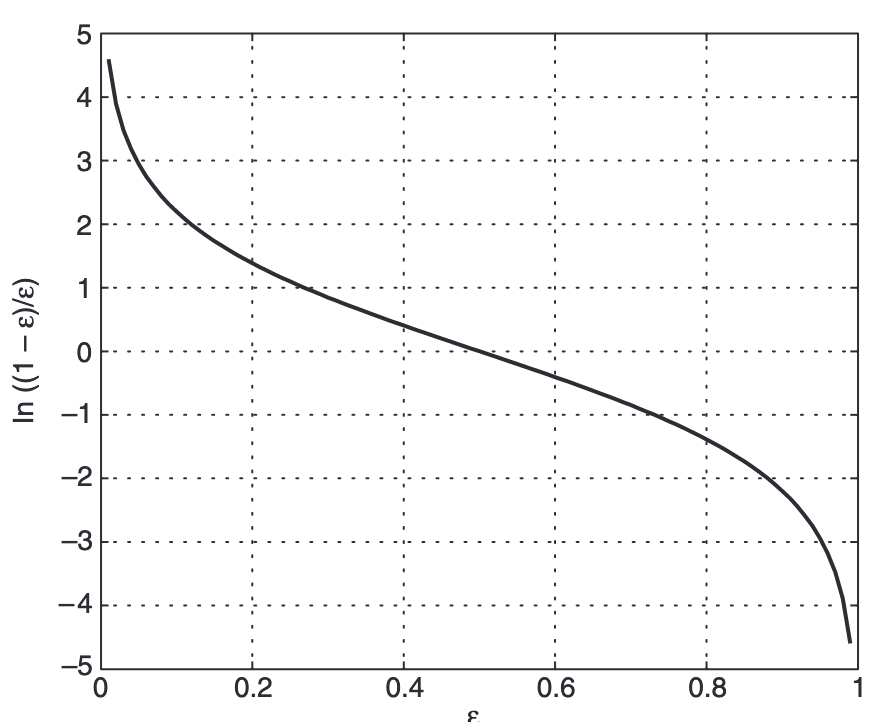
\includegraphics[width=\linewidth]{img/importance_vs_errorrate.png}
    \caption{$\alpha$ as a function of the error rate.}
    \label{fig:importance-errorrate}
\end{wrapfigure}


If  $\varepsilon_i\approx 0$, then $\alpha_i \gg0$, meaning that we will trust more this classifier; if $\varepsilon_i \approx 1$, then $\alpha_i \ll 0$.

The importance of a classifier is used to update the weights of the training examples: given $x_i$, its corresponding weight at boosting round $j+1$ is:
\begin{equation}
    w_i^{(j+1)} = \dfrac{w_i^{(j)}}{Z_j} \times \begin{cases}
        e^{-\alpha_j} & C_j(x_i) = y_i \\
        e^{\alpha_j} & C_j(x_i) \neq y_i 
    \end{cases}
\end{equation}
$Z_j$ is the \textit{normalization factor} that ensures $\sum_i w_i^{(j+1)} = 1$. The formula raises the weight of incorrectly classified examples and lowers it for correctly classified ones, scaled by how \textit{good} the classifier is.

The classification is also influenced by the importance of the classifier:
\begin{equation}
    C^*(x) = \arg\max_y \sum_{j=1}^T \alpha_j \delta(C_j(x) = y)
\end{equation}
This approach penalizes models with poor accuracy; additionally, if any intermediate boosting round produces an error rate higher than 50\%, the weights of the examples are reverted to their original value $\frac{1}{n}$, and the resampling procedure is repeated.

The difference from bagging is the $\alpha$ value in $C^*(x)$: here we have a weighted majority vote, where more important classifiers weigh more in the final decision, whereas bagging uses a plain majority vote.

\subsubsection{Decision Stumps}
A common choice of models used by AdaBoost is a forest of \textbf{decision stumps}, i.e., decision trees with only a root and two leaf nodes. Individually, they are weak learners and perform poorly, but in an ensemble, they can be highly effective.

In a forest of stumps, some contribute more to the final classification than others. Each stump is not built independently; the error of one influences the next.

Initially, all records are assigned equal weights. We search for the first stump, ignoring the weights since they are uniform. To select the best stump, we use the Gini Index (or entropy, or continuous attribute methods as in standard decision trees). We then compute its importance (\ref{AdaImportance}) in the final classification using its total error $\varepsilon_i$ (\ref{AdaErrorRate}).

\begin{wrapfigure}{r}{0.17\textwidth}
    \centering
    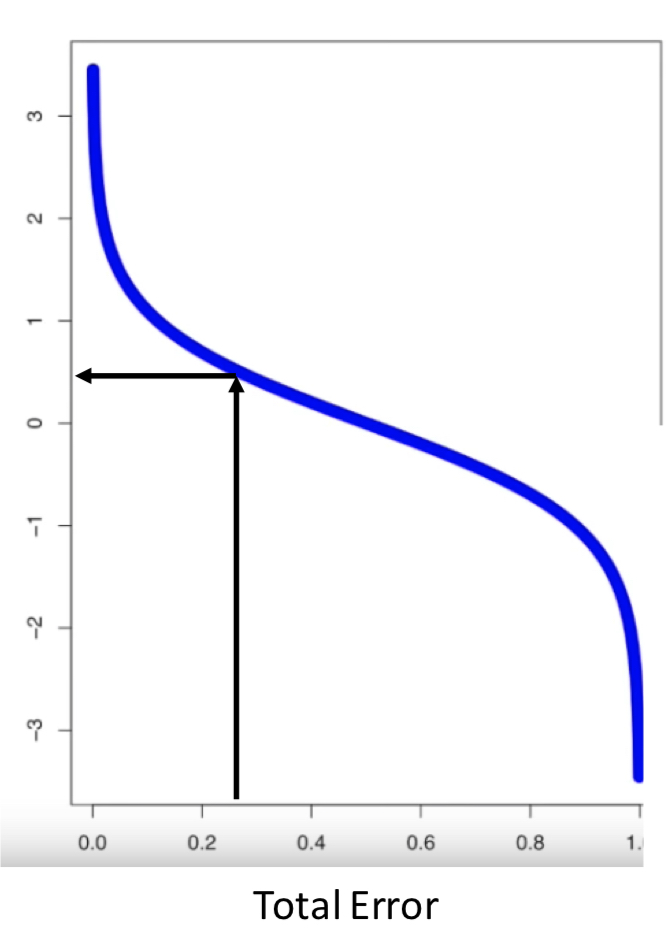
\includegraphics[width=\linewidth]{img/32_dm2_ensemble_2023_24.jpeg}
\end{wrapfigure}

Next, we update the sample weights to emphasize misclassified examples:
\begin{equation}
    w^{(t+1)} = w^{(t)} \times\ e^{\alpha_i}    
\end{equation}

The higher the importance $\alpha_i$, the more the weights of misclassified samples increase. Correctly classified samples have their weights decreased. Since models with error above 0.5 are discarded, $\alpha_i$ is always non-negative, and only the left portion of the image is used.

After updating, we normalize the weights so that their sum is 1, allowing them to be treated as probabilities. These new weights replace the old ones.

The updated weights are used to build the second stump. While in theory we could use weighted Gini Index, in practice we often generate a new dataset by duplicating samples according to their weights. This resampled dataset is then used to build the next stump, repeating the process.


\subsection{Random Forest}
\textbf{Random forests} enhance classifier performance by constructing an ensemble of decorrelated \textit{decision trees}. They aggregate the predictions of multiple trees and output the class that is the mode of the individual predictions. The term \textit{random} refers to the random subset of features considered, while \textit{forest} indicates the use of decision trees.

Each decision tree is built on a \textit{bootstrap sample} generated from independent random vectors. If all bootstrap samples used the same features, the resulting trees would be nearly identical, because the important features would dominate every tree; sampling the attributes at random breaks this and increases diversity. Bagging with decision trees is a special case of random forests, one where randomness is injected during model construction. Unlike AdaBoost, the random vectors are drawn from a fixed probability distribution.

A key characteristic is that each tree is trained on a subset of attributes, typically of size $m' \approx \sqrt{m}$ or $m' \approx \log(m)$. The trees are unpruned and grow until all leaves are pure. As a result, the base models have low bias but high variance.

They are among the most accurate learning algorithms available, and stay efficient even on large datasets with thousands of input variables, without requiring explicit feature selection. The model identifies the most relevant features on its own, estimates variable importance, and provides an internal, unbiased estimate of the generalization error as the forest is built.

\subsection{Gradient Boosting (GB)}
\textbf{Gradient Boosting} aims to find the best hypothesis by iteratively expanding an initial function.
\subsubsection{GB for Regression}
\begin{align}
    &F_0(x) = \arg \min_{\gamma} \sum_{i=1}^n L(y_i, \gamma) = \mathbb{E}[y] \\
    &F_m(x) = F_{m-1}(x) + \left( \arg \min_{h_m \in H} \sum_{i=1}^n L(y_i, F_{m-1}(x_i) + h_m(x_i)) \right)(x)
\end{align}

Here $h_m$ is a base learner and $L$ is the loss function, commonly the squared error loss $\frac{1}{2}(y - \hat{y})^2$. Differentiating it with respect to the predicted value yields the negative \textit{residual}, which simplifies the gradient-based updates.

In $F_0(x)$, the summation accounts for the loss over all observations, and $\arg\min_\gamma$ identifies the prediction that minimizes this loss: essentially the point minimizing the total squared residuals. This results in the mean of the targets, making $F_0(x)$ a constant (a single leaf).

Since directly finding the optimal function at each step is challenging, a steepest descent approach is used. After computing $F_0(x)$, the following steps are repeated:

\begin{enumerate}
    \item \textbf{Compute pseudo-residuals:} represent the gradients with respect to the current predictions.
    \begin{equation}
        r_{im} = -\left[ \dfrac{\partial L(y_i, F(x_i))}{\partial F(x_i)} \right]_{F(x) = F_{m-1}(x)}, \quad \forall i = 1, \dots, n
    \end{equation}
    \item \textbf{Fit a base learner} (e.g., a shallow decision tree) to the training set $\{x_i, r_{im}\}_{i=1}^n$, partitioning the space into \textbf{terminal regions} $R_{jm},\ j=1,\dots,J_m$.
    \item \textbf{Compute leaf values} which minimize the loss within each region, defining the leaf outputs.
    \begin{equation}
        \gamma_{jm} = \arg \min_{\gamma} \sum_{x_i \in R_{jm}} L(y_i, F_{m-1}(x_i) + \gamma)
    \end{equation}
    \item \textbf{Update the model } given $\nu$ learning rate, and $1(\cdot)$ indicator function
    \begin{equation}
        F_m(x) = F_{m-1}(x) + \nu \sum_{j=1}^{J_m} \gamma_{jm} \cdot 1(x \in R_{jm})
    \end{equation}
\end{enumerate}
\subsubsection{GB for Classification}
For \textbf{classification}, predictions are expressed as the log-odds of the positive class. To turn them into probabilities, we apply the logistic function:
\begin{equation}
\frac{e^{\log(p)}}{1 + e^{\log(p)}} = \frac{p}{1+p} \qquad note: p \text{ means odds}
\end{equation}
If the resulting probability exceeds 0.5, the instance is classified as positive.

\textbf{Pseudo-residuals} are computed as the difference between observed and predicted values. In regression a single residual directly determines the leaf value, but classification needs extra care because of the log-odds representation. Since leaves contain a mix of observations, the update values $\gamma_{jm}$ are computed as:
\begin{equation}
    \gamma_{jm} = \frac{\sum_{i \in R_{jm}} \text{Residual}_i}{\sum_{i \in R_{jm}} p_i (1 - p_i)}
\end{equation}
where $p_i$ is the previous probability estimate for sample $i$ and $R_{jm}$ represents the set of observations in region $j$ of tree $m$. The \textbf{log-likelihood of the observed data given the prediction} is:
\begin{equation}
    \sum_{i=1}^N \left[ y_i \log(p_i) + (1-y_i)\log(1-p_i) \right]  \qquad y_i \text{ observed value}
\end{equation}
By converting the negative log-likelihood into a function of the predicted log-odds, we obtain:
\begin{equation}
    -y_i \log(odds) + \log(1+e^{\log(odds)})
\end{equation}

Taking the derivative of this loss function with respect to the predicted log-odds gives:
\begin{equation}
    -y_i + \frac{e^{\log(odds)}}{1+e^{\log(odds)}} = -y_i + p_i
\end{equation}

After initializing $F_0$, we calculate pseudo-residuals as $y_i - p_i$ (difference between observed and predicted probabilities). In the subsequent steps, we build a regression tree and compute the optimal values for terminal regions:
\begin{equation}
    \gamma_{1,1} = \frac{\text{Residual}_1}{p_1 (1-p_1)} \qquad
    \gamma_{2,1} = \frac{\text{Residual}_2 + \text{Residual}_3}{p_2(1-p_2) + p_3(1-p_3)}    
\end{equation}
These values are then used to update predictions for each sample, completing one iteration of the boosting process.
\subsubsection{eXtreme Gradient Boosting (XGBoost)}

\textbf{XGBoost} is a regularized implementation of Gradient Boosting that improves performance and generalization. Unlike standard Gradient Boosting, which uses classical regression trees, XGBoost uses a special type of tree and introduces regularization during the tree construction.

\bigskip

\begin{enumerate}
    \item \textbf{Initial prediction.}  
    Training starts with an initial prediction $F_0(x)$, which is typically set to $0.5$ for both regression and classification. This serves as the baseline for computing residuals.

    \item \textbf{Tree initialization.}  
    A tree is initialized with a single leaf that contains all training instances. Residuals are computed based on the difference between observed and predicted values.

    \item \textbf{Compute similarity scores.}  
    The goal is to split the data such that we maximize the \textbf{gain} in similarity. The \textbf{similarity score} measures the quality of a potential leaf:
    \begin{itemize}
        \item \textbf{Regression:}
        \[
        \text{Similarity} = \frac{\left( \sum_i r_i \right)^2}{l + \lambda}
        \]
        where $r_i$ is the residual for sample $i$, $l$ is the number of samples in the leaf, and $\lambda$ is a regularization parameter.
        
        \item \textbf{Classification:}
        \[
        \text{Similarity} = \frac{\left( \sum_i r_i \right)^2}{\sum_i p_i (1 - p_i) + \lambda}
        \]
        where $p_i$ is the predicted probability for instance $i$.

        \item In both cases, the denominator (excluding $\lambda$) is referred to as the \textit{cover}, representing the effective number of observations in the leaf.
    \end{itemize}

    \item \textbf{Evaluate candidate splits.}
    For each possible split, compute the \textbf{gain}:
    \[
    \text{Gain} = \text{Similarity}_{\text{left}} + \text{Similarity}_{\text{right}} - \text{Similarity}_{\text{parent}}
    \]
    The split that maximizes this gain is selected. This process is repeated recursively to grow the tree until a maximum tree depth is reached (default is 6), or a leaf contains only one sample.

    \item \textbf{Pruning (regularization with $\gamma$).}  
    Once the tree is fully grown, it is pruned based on a threshold $\gamma$: if the gain of a node is less than $\gamma$, it is pruned. This avoids overfitting by removing branches that do not provide a sufficient gain.  
    A higher $\lambda$ generally leads to lower similarity scores, making pruning more likely.

    \item \textbf{Update the prediction.}  
    After building the tree, each instance receives an updated prediction:
    \[
    F_m(x) = F_{m-1}(x) + \eta \cdot \text{Tree}_m(x)
    \]
    where $\eta$ is the learning rate (default $\eta = 0.3$), and $\text{Tree}_m(x)$ is the tree's output for instance $x$.

    \item \textbf{Output value in a leaf.} The output value for a leaf is:
    \[
    \text{Output value} = \frac{\sum_i r_i}{l + \lambda}
    \]
    If $\lambda = 0$, this reduces to the unregularized average of residuals. Increasing $\lambda$ shrinks the output, reducing the influence of individual data points.
\end{enumerate}

\bigskip

\noindent \textbf{Note (for classification):}
As in regular Gradient Boosting, predictions are made on the log-odds scale. After computing the output of the tree, we add it to the previous log-odds prediction:
\[
F_m(x) = F_{m-1}(x) + \eta \cdot \text{Tree}_m(x)
\]
Then we convert the result to a probability via the logistic function:
\[
p(x) = \frac{1}{1 + e^{-F_m(x)}}
\]
The model keeps adding trees until either the maximum number of iterations is reached or the residuals become negligibly small.


\subsubsection{LightGBM}
\textbf{LightGBM} is a high-performance implementation of Gradient Boosting developed by Microsoft. It is designed to be faster and more memory-efficient than traditional implementations such as XGBoost, while maintaining comparable accuracy.

\begin{itemize}
    \item It uses \textbf{Histogram-based Gradient Boosting}, which discretizes continuous feature values into $k$ bins. This reduces computation and memory usage, enabling faster training.
    
    \item It supports \textbf{parallel learning} and \textbf{GPU acceleration}, improving scalability on large datasets.
    
    \item Trees produced by LightGBM often exhibit more \textbf{vertical growth} (i.e., deeper trees) compared to XGBoost, which tends to grow \textbf{horizontally} (wider trees).

    \item LightGBM implements two key optimizations:
    \begin{enumerate}
        \item \textbf{Gradient-based One-Side Sampling (GOSS)}:  
        During training, data points with large gradients (i.e., poorly predicted) are retained, while those with small gradients are randomly subsampled. This reduces computation while preserving accuracy.

        \item \textbf{Exclusive Feature Bundling (EFB)}:  
        A technique to reduce the number of input features by combining mutually exclusive features (those that never take non-zero values at the same time) into a single feature.
    \end{enumerate}

    \item LightGBM natively handles \textbf{categorical features} and \textbf{missing values}.
\end{itemize}

\subsubsection{CatBoost (Categorical Boosting)}

\textbf{CatBoost} is a Gradient Boosting framework developed by Yandex, specifically optimized for datasets with many categorical variables. It introduces several innovations to handle these cases effectively:

\begin{itemize}
    \item \textbf{Ordered Target Encoding}:  
    encodes categories using statistics derived from the target variable, while preventing target leakage by computing them in an ordered manner during training.
    \item Builds \textbf{Symmetric Decision Trees}:  
    all nodes at the same depth share the same splitting condition. This makes tree traversal more efficient and improves GPU performance.
    \item Like LightGBM and XGBoost, it supports missing values and categorical inputs natively.
\end{itemize}

\subsubsection{Explainable Boosting Machines (EBM)}

\textbf{Explainable Boosting Machines} are a class of models based on \textbf{Generalized Additive Models (GAMs)}. Unlike traditional black-box models, EBMs are designed to be fully interpretable.

\begin{itemize}
    \item EBMs model the outcome as a sum of univariate functions, trained one feature at a time in a round-robin fashion: $y = f_1(x_1) + f_2(x_2) + \dots + f_n(x_n)$
    
    \item This contrasts with:
    \begin{itemize}
        \item \textbf{Linear models:} \( y = \beta_1 x_1 + \dots + \beta_n x_n \)
        \item \textbf{Complex models:} \( y = f(x_1, \dots, x_n) \)
    \end{itemize}
\end{itemize}

EBMs can incorporate pairwise interactions when necessary, but the additive structure ensures that each feature's effect can be visualized and understood independently.

They are used in high-stakes domains such as healthcare and finance, where interpretability matters as much as accuracy.
